\section{Durchführung und Aufbau}
\label{sec:Durchführung}
Die im Versuch verwendete Apparatur besteht aus einem Geiger-Müller-Zählrohr, auf das die aktivierte Probe gesteckt wird.
Das Zählrohr ist hierbei dank einer Bleiabschirmung besonders gut von der Umgebungsstrahlung (Nulleffekt) abgeschirmt. Dies
ist sehr wichtig, da die Anzahl der einzelnen gemessenen Zerfälle sehr klein sein können.\\
Die Zählung der Zerfälle erfolgt, nach Signalweitergabe des Zählrohrs, mithilfe eines umschaltbaren Zählwerks, dass jeweils nach einem
festlegbaren Intervall zwischen zwei Impulszählern hin und her schaltet, was einfaches Ablesen und eine kontinuierliche Messung
ermöglicht.\\
Der verwendete Versuchsaufbau ist in \autoref{Abb:Versuchsaufbau} zu sehen.
\begin{figure}
    \centering
    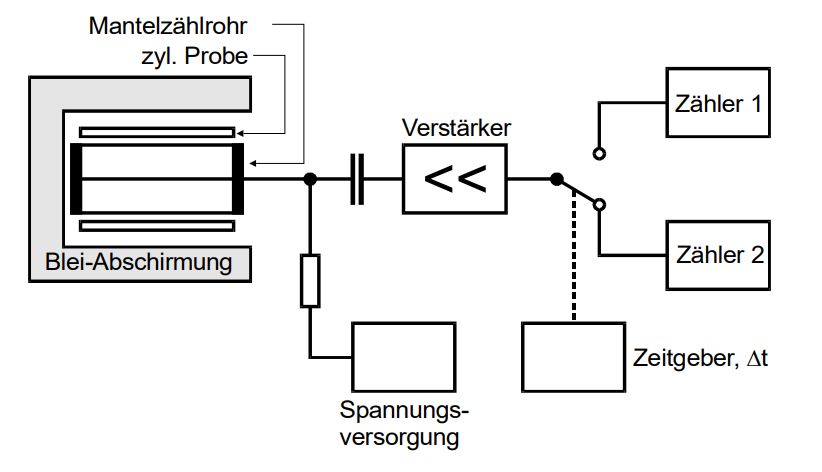
\includegraphics[width=15cm]{Bilder/Versuchsaufbau.png}
    \caption{Verwendeter Versuchsaufbau zum Zählen der Zerfälle.\cite{sample}}
    \label{Abb:Versuchsaufbau}
\end{figure}

\subsection{Aktivierung der Atomkerne durch Neutronenbeschuss}

Die Proben werden in einer speziellen Apparatur mit langsamen Neutronen beschossen und dadurch aktiviert.\\
Diese Apparatur ist mit Paraffin (bestehend aus gesättigten Kohlenwasserstoffen) gefüllt, um die durch Kernreaktionen
entstandenen Neutronen so stark wie möglich abzubremsen, bevor sie auf die Proben treffen. Die verwendete 
Apparatur ist ist \autoref{Abb:Aktivierung} dargestelllt.

\begin{figure}
    \centering
    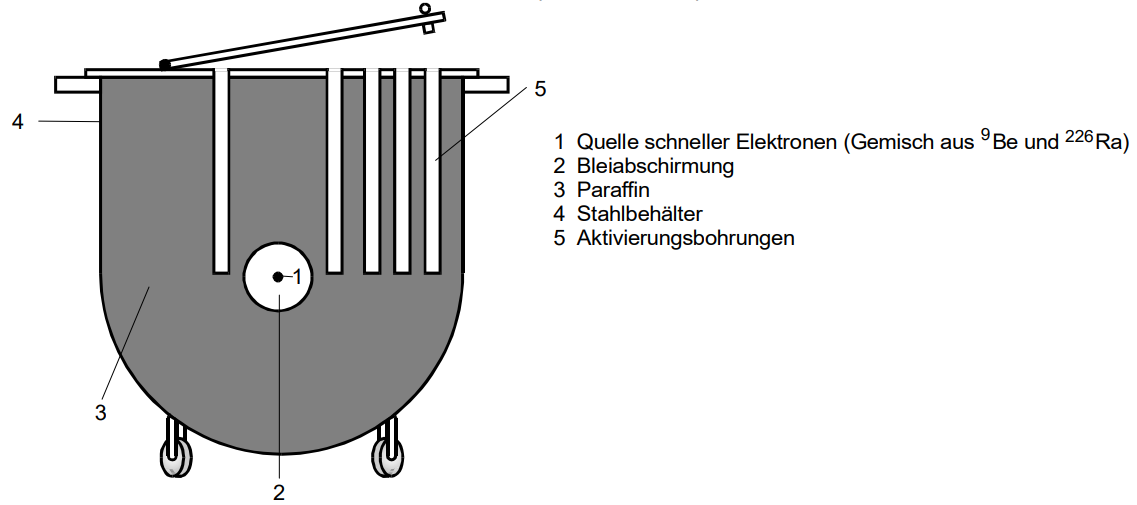
\includegraphics[width=15cm]{Bilder/Aktivierung.png}
    \caption{Verwendeter Versuchsaufbau zur Aktivierung der Proben.\cite{sample}}
    \label{Abb:Aktivierung}
\end{figure}

\subsection{Bestimmung der Halbwertszeit der aktivierten Isotope}

Zu Beginn wird eine Nullmessung über 500 s durchgeführt, um den Nulleffekt zu bestimmen.\\
Die aktivierten Proben müssen nach dem Entfernen aus dem Stahlbehälter mit Paraffin so schnell wie möglich in die Messapparatur
eingebracht werden, um die Halbwertszeit so genau wie möglich bestimmen zu können.\\
Es wird jeweils eine Messreihe für das Isotop $\isotope[52][]{V}$ (Vanadium) und das Isotopengemisch $\isotope[108][]{Ag}$ und 
$\isotope[110][]{Ag}$ (Silber) durchgeführt.\\
Zuerst werden bei dem Vanadium jeweils 30 Messungen gemacht, welche jeweils 30 Sekunden lang sind. Also wurde das Isotop
insgesamt über 15 Minuten hinweg beobachtet.\\
Anschließend werden bei dem Silber 42 Messungen, jeweils zehn Sekunden lang, durchgeführt. Das ergibt hier eine Gesamtzeit von sieben Minuten.\\